\documentclass{beamer}

\setlength{\unitlength}{1cm} 
\usetheme{Madrid}

\usepackage[english]{babel}
\usepackage[utf8]{inputenc}

\usepackage{amsmath, amssymb, mathtools, bbm}
\usepackage{bm}

\usepackage{graphicx}
\usepackage{wrapfig}
\usepackage{tikz} 
\usepackage{relsize}
\usepackage{makecell}
\usepackage{booktabs}
\usepackage{subcaption}
\usepackage{float}
\usepackage{multirow} 

\usepackage[style=apa]{biblatex}
\usepackage{csquotes}

\bibliography{
    ../../../../Desktop/bibliographies/thesis,
    ../maths}


% Graphs
\usetikzlibrary{positioning, arrows.meta, calc, decorations.markings, math, matrix, fit, backgrounds}

\tikzset{fontscale/.style = {font=\relscale{#1}}}

\definecolor{prosumer}{cmyk}{0,0.816,0.408,0}

% Math commands
\newcommand{\E}{\mathbb{E}}
\newcommand{\R}{\mathbb{R}}
\newcommand{\B}{\mathbb{B}}

\newcommand{\matr}[1]{\bm{#1}}
\newcommand{\set}[1]{\left\{#1\right\}}

\newcommand{\Y}{\matr{Y}}
\newcommand{\I}{\matr{I}}
\newcommand{\G}{\matr{G}}
\newcommand{\T}{\matr{T}}

\newcommand{\V}{\mathbb{V}}


\title{How directed is a directed network?}
\author{Andrea Titton}
\title{Thesis defence}
\subtitle{Contagion of Electricity Prices \\ A Dynamic Game of Price Hikes Propagation}
\institute{Tinbergen Institute}
\date{04/12/2020}

\begin{document}

\frame{\titlepage}

\begin{frame}{Motivation}
    Green energy transition and advent of \textbf{prosumers}
    \vspace{2em}
    \begin{itemize} \setlength\itemsep{1.5em}
              \pause \item Risk of \textit{local} demand shocks
              \pause \item \textbf{Local quasi-monopolies} energy providers (e.g. ERCOT case in Texas) and decentralized prosumers
              \pause \item Weather shocks lead to \textbf{uncertainty} among risk averse consumers
    \end{itemize}
\end{frame}

\begin{frame}{Lack of price convergence}
    \begin{figure}
        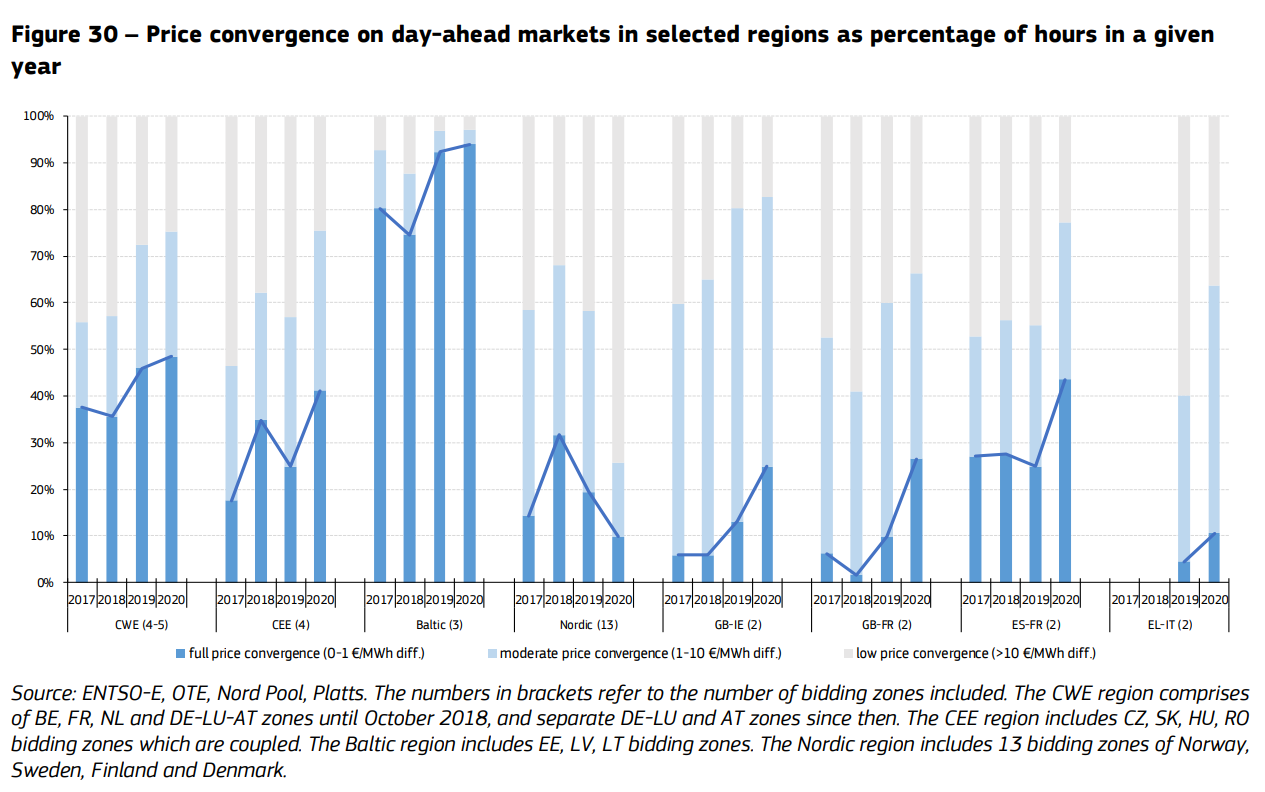
\includegraphics[height = 0.7\textheight]{figures/convergence.PNG}
        \caption{\cite{Report2019}}
    \end{figure}
\end{frame}

\begin{frame}{Research question}

    Prosumers induce three sources of uncertainty: bounded rationality, risk aversion, and renewable energy volatility

    \begin{itemize} \setlength{\itemsep}{1em}
        \item \textit{How do exogenous and unexpected demand shocks affect the price formation mechanism?} \pause
        \item \textit{How do shock in prices transmit to the cross-border market?} \pause
        \item \textit{Hysteresis: can this shock produce sustained price imbalances?} \pause
        \item \textit{Are current policies effective in this framework?}
    \end{itemize}

\end{frame}

\begin{frame}{What is new?}

    Comparison with previous ABM (\cite{Weidlich2008})
    \vfill

    \visible<1->{\begin{minipage}{0.4\textwidth}
            \resizebox{\textwidth}{!}{\tikzstyle{basic} = [
draw,circle,
minimum size=10pt,
]

\tikzstyle{core} = [
draw,circle,
minimum size=10pt,
prosumer,
fill=prosumer,
text=black
]

\begin{tikzpicture}[-{Latex[scale=1]}, thick]

    \node [core] (1) {Consumers};
    \node [core, below = 4cm of 1] (3) {Producers};
    \node [basic, right = 1cm of 1] (2-1) {\makecell[c]{Constant \\ demand}};
    \node [basic, right = 1cm of 3] (4) {\makecell[c]{Market \\ power}};
    \node [basic, above = 1cm of 4] (2-2) {Supply};
    \node [basic, below right = 1cm and 2cm of 2-1] (5) {Prices};


    \path
    (1) edge (2-1)
    (4) edge (2-2)
    (3) edge (4)
    (2-2) edge (5)
    (2-1) edge [dashed, -] (5)
    ;

\end{tikzpicture}}
        \end{minipage}}
    \hfill
    \visible<2->{\begin{minipage}{0.55\textwidth}
            \resizebox{\textwidth}{!}{\tikzstyle{basic} = [
draw,circle,
minimum size=10pt
]

\tikzstyle{core} = [
draw,circle,
minimum size=10pt,
prosumer,
fill=prosumer,
text=black
]


\begin{tikzpicture}[-{Latex[scale=1]}, thick]

    \node [core] (1) {Prosumers};
    \node [core, below = 4cm of 1] (3) {Producers};
    \node [basic, right = 1cm of 1] (2-1) {\makecell[c]{Demand \\ shocks}};
    \node [basic, right = 1cm of 3] (4) {\makecell[c]{Market \\ power}};
    \node [basic, above = 1cm of 4] (2-2) {\makecell[c]{Supply \\ shocks}};
    \node [basic, below right = 1cm and 2cm of 2-1] (5) {Prices};
    \node [basic, right = 1cm of 4] (7) {\makecell[c]{Bargaining \\ power}};
    \node [core, right = 1cm of 7] (6) {Providers};


    \path
    (1) edge (2-1)
    (4) edge (2-2)
    (3) edge (4)
    (2-2) edge (5)
    (2-1) edge (5)
    (6) edge (7)
    (7) edge (4) 
    ;

\end{tikzpicture}}
        \end{minipage}}
\end{frame}

\begin{frame}{Model outline}
    \centering
    \only<1>{
        \resizebox{\textwidth}{!}{\tikzstyle{var} = [
draw,circle,
prosumer,
fill=prosumer,
text=black,
minimum size=10pt]

\tikzstyle{agent} = [
draw, circle,
fill=blue!30,
minimum size=10pt]

\tikzstyle{derived} = [
draw, circle, dashed,
minimum size=10pt]

\tikzstyle{time} = [
draw=gray, rectangle,
dashed,
thick,
inner sep=5pt]

\tikzstyle{market} = [
draw=gray, circle,
dashed,
thick,
inner sep=5pt]


\begin{tikzpicture}[-{Latex[scale=1]}, thick, every text node part/.style={align=center, fontscale=0.8}]

    \node [agent] (prov) {Provider};
    \node [market, left = 2cm of prov] (cb-market) {Cross-border \\ market};
    \node [agent, above right = 1cm and 5cm of prov] (prod) {Producers};
    \node [agent, below right = 1cm and 5cm of prov] (pros) {Prosumers};
    \node [market, right = 2cm of prov] (w-market) {Local \\ wholesale \\ market};

    \path
    (cb-market) edge [bend left] node [above] {$Y_t$} (prov)
    (prov) edge [dashed, bend left] node [below] {$P_t$} (cb-market)
    (prov) edge [ bend left] node [above] {$X_t$} (w-market)
    (w-market) edge [dashed, bend left] node [below] {$p_t$} (prov)
    (prod) edge [] node [above left] {$S_t$} (w-market)
    (w-market) edge [{Latex[scale=1]}-{Latex[scale=1]}] node [below left] {$e_t \  M$} (pros)
    ;

\end{tikzpicture}}}
    \only<2>{
        \resizebox{\textwidth}{!}{\tikzstyle{var} = [
draw,circle,
prosumer,
fill=prosumer,
text=black,
minimum size=10pt]

\tikzstyle{agent} = [
draw, circle,
fill=blue!30,
minimum size=10pt]

\tikzstyle{derived} = [
draw, circle, dashed,
minimum size=10pt]

\tikzstyle{time} = [
draw=gray, rectangle,
dashed,
thick,
inner sep=5pt]

\tikzstyle{market} = [
draw=gray, circle,
dashed,
thick,
inner sep=5pt]


\begin{tikzpicture}[-{Latex[scale=1]}, thick, every text node part/.style={align=center, fontscale=0.8}]

    \node [agent] (prov) {Provider};
    \node [market, left = 2cm of prov] (cb-market) {Cross-border \\ market};
    \node [agent, above right = 1cm and 5cm of prov] (prod) {$N$ Producers};
    \node [agent, below right = 1cm and 5cm of prov] (pros) {$M$ Prosumers};
    \node [market, right = 2cm of prov] (w-market) {Local \\ wholesale \\ market};

    \path
    (cb-market) edge [bend left] node [above] (Y) {$Y_t$} (prov)
    (prov) edge [dashed, bend left] node [below] (P) {$P_t$} (cb-market)
    (prov) edge [ bend left] node [above] (X) {$X_t$} (w-market)
    (w-market) edge [dashed, bend left] node [below] (p) {$p_t$} (prov)
    (prod) edge [] node [above left] (S) {$S_t$} (w-market)
    (w-market) edge [{Latex[scale=1]}-{Latex[scale=1]}] node [below left] (e) {$e_t$} (pros)
    ;

    \node[draw, dotted, outer sep = 0, inner sep = 0, fit = (w-market) (e) (p) (X) (S) (prod) (pros)]{};

\end{tikzpicture}}}
\end{frame}

\begin{frame}{Prosumers}
    \begin{itemize} \setlength\itemsep{1.5em}
        \item M producer pre local market \pause
        \item All with the same ``demand endowment'' $e_t$
    \end{itemize}
\end{frame}

\begin{frame}{Producers setup}
    Main modelling assumption \vspace{5mm}
    \begin{itemize} \setlength\itemsep{1.5em}
        \item Price takers $p_t$ and oligopolist \pause
        \item Produce electricity $s_t$ at fixed marginal cost $k$ \pause
        \item Can ramp-up or down production with a period delay by $r_t \in [\underline{r}, \overline{r}]$ \pause
        \item This costs them $c(s_t, r_t)$
    \end{itemize}
\end{frame}


\begin{frame}{Producers optimization}
    \begin{equation*}
        V(s_t, p_t) = \max_{r_t} \left\{ s_t \ \underbrace{(p_t - k)}_{\text{unit profit}} - \underbrace{ c(s_t, r_t) \  r_t }_{\text{ramp-up costs}} + \beta \  V(s_{t+1}, p_{t+1}) \right\}
    \end{equation*}
    \vspace{5mm}
    \visible<2>{\begin{itemize} \setlength\itemsep{1.5em}
            \item $s_{t+1} = s_t + r_t$
            \item Providers are naive: $\B[p_{t+1}] = p_t$
        \end{itemize}}
\end{frame}

\begin{frame}

    \visible<1->{
        \begin{equation*}
            mc = \overbrace{c(s_t, r)}^{\text{cost you pay today}} + \overbrace{r \frac{\partial c}{\partial r}(s_t, r)}^{\text{moved to new cost level}}
        \end{equation*}
    }

    \visible<2>{
        \begin{equation*}
            \begin{split}
                \frac{mb}{\beta} &= \overbrace{(p_t - k)}^{\text{unit profit}} + \overbrace{\left(\frac{\partial c}{\partial r}(s_t + r, r) - \frac{\partial c}{\partial s_t}(s_t + r, r)\right)}^{\text{moved to a new level of costs tomorrow}} \ r + \\
                & + \underbrace{c(s_t + r, r)}_{\text{costs you do not pay tomorrow}}
            \end{split}
        \end{equation*}
    }

\end{frame}

\begin{frame}
    \begin{figure}
        \includegraphics[width = 0.8 \textwidth]{../../plots/rfunction.pdf}
    \end{figure}
\end{frame}

\iffalse
    % CB market
    \begin{frame}{Model outline}
        \centering
        \only<1>{
            \resizebox{\textwidth}{!}{\tikzstyle{var} = [
draw,circle,
prosumer,
fill=prosumer,
text=black,
minimum size=10pt]

\tikzstyle{agent} = [
draw, circle,
fill=blue!30,
minimum size=10pt]

\tikzstyle{derived} = [
draw, circle, dashed,
minimum size=10pt]

\tikzstyle{time} = [
draw=gray, rectangle,
dashed,
thick,
inner sep=5pt]

\tikzstyle{market} = [
draw=gray, circle,
dashed,
thick,
inner sep=5pt]


\begin{tikzpicture}[-{Latex[scale=1]}, thick, every text node part/.style={align=center, fontscale=0.8}]

    \node [agent] (prov) {Provider};
    \node [market, left = 2cm of prov] (cb-market) {Cross-border \\ market};
    \node [agent, above right = 1cm and 5cm of prov] (prod) {$N$ Producers};
    \node [agent, below right = 1cm and 5cm of prov] (pros) {$M$ Prosumers};
    \node [market, right = 2cm of prov] (w-market) {Local \\ wholesale \\ market};

    \path
    (cb-market) edge [bend left] node [above] (Y) {$Y_t$} (prov)
    (prov) edge [dashed, bend left] node [below] (P) {$P_t$} (cb-market)
    (prov) edge [ bend left] node [above] {$X_t$} (w-market)
    (w-market) edge [dashed, bend left] node [below] {$p_t$} (prov)
    (prod) edge [] node [above left] {$S_t$} (w-market)
    (w-market) edge [{Latex[scale=1]}-{Latex[scale=1]}] node [below left] {$e_t$} (pros)
    ;

    \node[draw, dotted, fit = (cb-market) (Y) (P)]{};

\end{tikzpicture}}}
        \only<2>{
            \resizebox{!}{0.7\textheight}{\tikzstyle{prosumers} = [
draw,circle,
prosumer,
fill=prosumer,
text=black,
minimum size=5pt]

\tikzstyle{provider} = [
draw,circle,
minimum size=10pt]

\tikzstyle{market} = [
draw=gray, dashed, thick,
inner sep=8pt]


\begin{tikzpicture}[{Latex[scale=0.5]}-{Latex[scale=0.5]}, thick]

    % Placing providers
    \foreach \x/\y [count=\j] in {1/1, -1/1, 1/-1, -1/-1}
        % Draw provider
        {\node [provider]  (\j) at (2*\x, 2*\y) [fontscale=0.8] {\makecell[l]{Prov. \j \\ $X(p_{\j})$}};

            % Draw prosumers
            \edef\points{}
            \foreach \z/\w [count=\i] in {0/2, 1/2.1, 1.75/1.75, 2.1/1, 2/0}
                {\node [prosumers] (\x\y\i) at (\x + 1.3*\x*\z, \y + 1.5*\y*\w) [fontscale=0.6] {$x_{\i}$};
                    \path (\j) edge [] node [fontscale = 0.6] {} (\x\y\i);
                    \xdef\points{(\x\y\i) \points}
                };}

    \path
    (1) edge [-{Latex}] node [above, fontscale=0.8] {$Y^{(1, 2)}$} (2)
    (1) edge [-{Latex}] node [right, fontscale = 0.8] {$Y^{(1, 3)}$} (3)
    (1) edge [-{Latex}] node [above left, fontscale = 0.8] {$Y^{(1, 4)}$} (4)
    (3) edge [-{Latex}] node [above, fontscale = 0.8] {$Y^{(3, 4)}$} (4);

\end{tikzpicture}}}
    \end{frame}
\fi


\begin{frame}[allowframebreaks]{Bibliography}
    \printbibliography
\end{frame}

\end{document}